\begin{Schunk}
\begin{Sinput}
> library("Ham94", lib.loc = "../../../library")
\end{Sinput}
\end{Schunk}
Finally we use similar techniques to calculate the effects of an impulse on a second order system.
Here each column of phi represents the coefficients of a second order system.
\begin{Schunk}
\begin{Sinput}
> T <- 20
> w <- 1 * (1:20 == 3)
> y <- array(dim = c(T, 2))
> y[1:2, ] <- 0
> phi <- array(c(0.6, 0.2, 0.5, -0.8), c(2, 2))
> for (j in 3:T) y[j, ] <- apply(X = phi * y[(j - 1):(j - 2), ], 
+     MARGIN = 2, FUN = sum) + w[j]
\end{Sinput}
\end{Schunk}
The results can be plotted reproducing figure 1.4.
\begin{center}
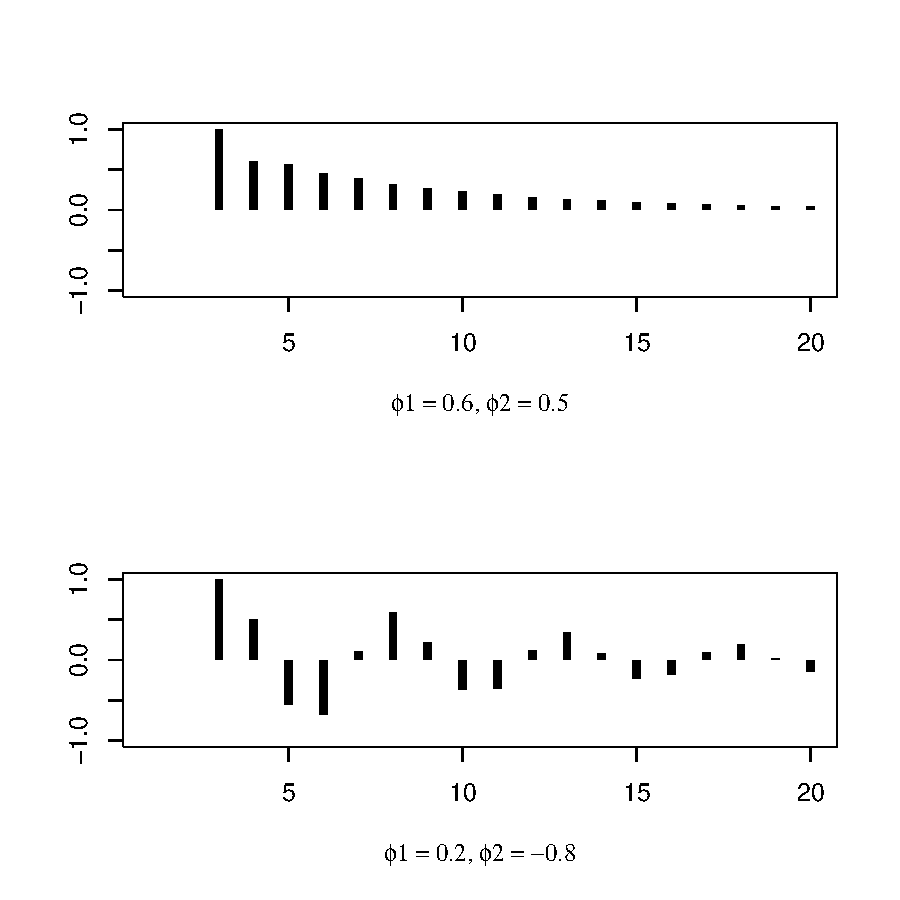
\includegraphics{p15-003}
\end{center}
